\documentclass[../main.tex]{subfiles}
\graphicspath{{\subfix{../Figures/}}}
\begin{document}
    \begin{frame}{Why mixing is hard in hypergraphs?} 
        \begin{itemize}
        	\item Proving mixing in hypergraphs is harder because it is not possible to define an equivalent discrete diffusion process as a random walk.
        	\item This is because the Laplacian is a non-linear operator, for $B_e$ the convex hull of $\{\chi_v-\chi_u : u,v\in e\}$ \cite{continuous_laplacian_hypergraph}:
	        	\begin{columns}
	        		\column{0.8\textwidth}
	        		\begin{block}{Laplacian for hypergraphs}
	        			$ \mathcal{L}(\bold{x}) = \{\sum_{e\in E} w_e \bold{b}_e\bold{b}_e^T \bold{x} \mid \bold{b}_e = \argmax_{\bold{b}\in B_e} \bold{x}^T\bold{b} \}$
	        		\end{block}
	        	\end{columns}
	        \item Such a laplacian operator is only good for describing $\frac{d \bold{p}_t}{d t} = -\mathcal{L}(D^{-1}\bold{p}_t)$ for infinitesimal time steps, hence the diffusion process is inherently continuous and harder to handle.
	        \item Observation: notice that the laplacian is a singleton matrix when the vector $\frac{\bold{p}_t}{\bold{d}}$ has piece-wise unique entries. The problem is handling ties. 	
        \end{itemize}
    \end{frame}
		
	\begin{frame}{Discrete diffusion process}
		\begin{itemize}
			\item Idea: turn the hypergraph laplacian into a singleton matrix by solving ties \textit{arbitrarily}. 
			\item Question: is this simple resolution of ties enough in order to obtain a diffusion process with good mixing properties?
		\end{itemize}
	\end{frame}

	\begin{frame}{Discrete diffusion process}
		\begin{itemize}
			\item We collapse the hypergraph $H$ into a multigraph $G_t$ at every time step, by collapsing every hyperedge $e$ into $(v_{\text{max}}^t(e), v_{\text{min}}^t(e))$
				\begin{columns}
					\column{0.8\textwidth}
					\begin{block}{$v_{\text{max}}^t(e)$}
						$v_{\text{max}}^t(e) = u\in e : \argmax_{u\in e} \frac{p_t(u)}{d(u)}$
					\end{block}
					\begin{block}{$v_{\text{min}}^t(e)$}
						$v_{\text{min}}^t(e) = u\in e : \argmin_{u\in e} \frac{p_t(u)}{d(u)}$
					\end{block}
					ties are solved by vertex index (smallest first).
				\end{columns}
			\item Self loops are added in order to preserve the degree of every node.
		\end{itemize}
	\end{frame}

	\begin{frame}{Discrete diffusion process}
		\begin{itemize}
			\item Since $G_t$ is a graph, it is possible to evolve the probability vector $\bold{p}_{t+dt} = M_t \bold{p}_t$. Notice that the step size is $dt\leq \frac{1}{2}$
			\item How to prove good mixing properties? We need to make sure that the sweep cuts $S_j(\bold{p}_{t+dt})$ has the same conductance $\hat{\phi}$ in the collapsed graph $G_t$ and in the original hypergraph $H$.
			\item Since the graph $G_t$ was made using the probability vector $\bold{p}_{t}$, the conductance of the sweep cut $S_j(\bold{p}_{t+dt})$ is not ensured to be preserved in $G_t$.
			\item Idea is to build a support $\tilde{G}_t$ collapsed graph, such that the conductance of the sweep cut $S_j(\bold{p}_{t+dt})$ in $\tilde{G}_t$ is preserved.
		\end{itemize}
	\end{frame}

	\begin{frame}{Discrete diffusion process}
		The proof of the mixing result goes like this:
		\begin{itemize}
				\item First, prove that the LS-curve $\tilde{I}_t$ is smaller than $I_t$. 
				\begin{lemma}
					\label{lemma:ls_curve_smaller_ls_curve_tilde}
					$\forall t$, 
					$I_{t+dt}(k) \leq \tilde{I}_{t+dt}(k)$
				\end{lemma} 
			\item Then, take advantage of the known conductance of the sweep cuts in $\tilde{G}_t$ to prove
				\begin{lemma}
					\label{lemma:recursive_LS_lower_bound}
					$\tilde{I}_{t+1}(k) \leq (1-2dt) I_t(k) + 2dt (I_t(k-\hat{\phi} \hat{k}) + I_t(k + \hat{\phi}\hat{k}))$
				\end{lemma}
			\item Which allows us to claim
				\begin{lemma}
					\label{lemma:mixing_result} 
					$I_t(k) - \pi(S_j(\bold{p}_t)) \leq \sqrt{k} e^{-t \hat{\phi}^2}$
				\end{lemma}
		\end{itemize}
	\end{frame}

	% proofs.
	\begin{frame}{Definition of $\tilde{G_t}$}
		How can be sure that the conductance of the sweep cut $S_j(\bold{p}_{t+dt})$ is preserved in $\tilde{G}_t$?
		
		\begin{itemize}
			\item $\forall e\in E$, if $(v_{\text{min}}^{t+dt}(e), v_{\text{max}}^{t+dt}(e))$ crosses the cut and $(v_{\text{min}}^{t}(e), v_{\text{max}}^{t}(e))$ does not, then either $(v_{\text{min}}^{t+dt}(e), v_{\text{min}}^{t}(e))$ or $(v_{\text{max}}^{t+dt}(e), v_{\text{max}}^{t}(e))$ also crosses the cut.
			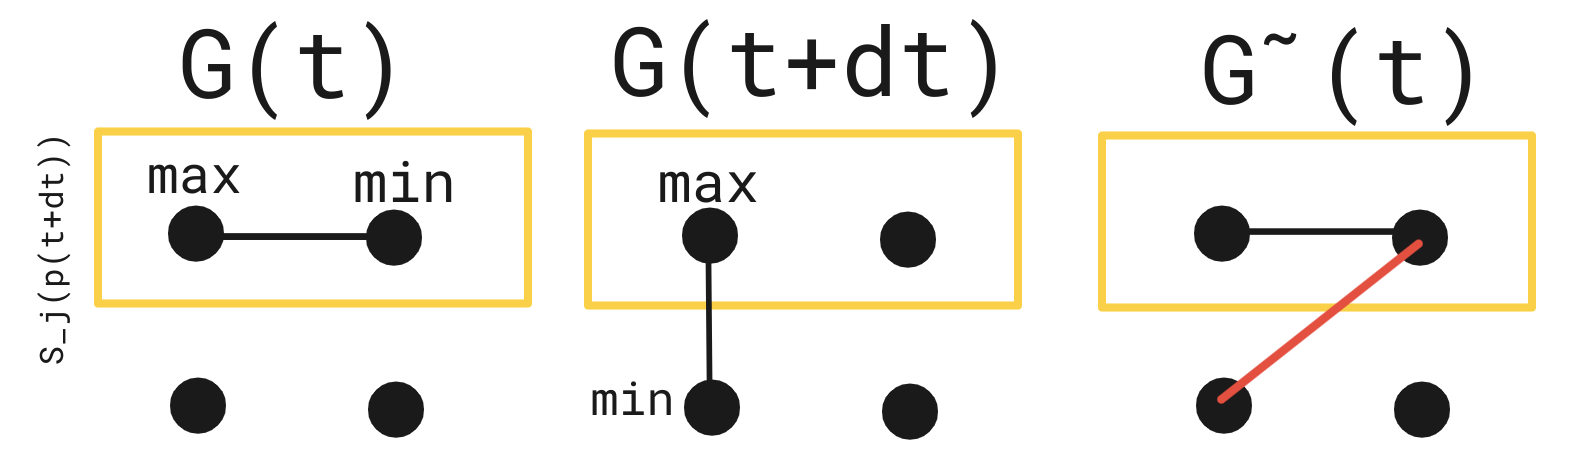
\includegraphics[width=0.8\textwidth]{Figures/G_tilde_creation}
			\item We can add to $G_t$ the new crossing collapsed edge, and remove enough self loops so that the degree of $\tilde{G}_t$ is the same as in $H$.
			\item We can now define $\tilde{\bold{p}}_{t+dt} = \tilde{M}_t \bold{p}_t$, and accordingly $\tilde{I}_{t+dt}$
		\end{itemize}
	\end{frame}

	\begin{frame}{Proof of Lemma \ref{lemma:ls_curve_smaller_ls_curve_tilde}}
		\begin{block}{Lemma \ref{lemma:ls_curve_smaller_ls_curve_tilde}}
			$\forall k\in[0,\text{vol}(H)], \forall t, I_{t+dt}(k) \leq \tilde{I}_{t+dt}(k)$
		\end{block}
		\begin{proof}
			The idea is that $\forall u\in S_j(\bold{p}_{t+dt})$, the new edges $(u,v)$ added to $\tilde{G}_t$ are such that $v$ has higher $\frac{p_t(v)}{d(v)}$ value than $\frac{p_t(u)}{d(u)}$. This ensures that the probability at time $t+dt$ on $u\in S_j(\bold{p}_{t+dt})$ is higher, and hence $\tilde{I}_{t+dt}(k) \geq I_{t+dt}(k)$.
		\end{proof}
	\end{frame}

	\begin{frame}{Proof of Lemma \ref{lemma:recursive_LS_lower_bound}}
		\begin{block}{Lemma \ref{lemma:recursive_LS_lower_bound}}
			$\tilde{I}_{t+dt}(k)\leq (1-2dt)I_t(k) + dt(I_t(k-\hat{\phi}\hat{k}) + I_t(k+\hat{\phi}\hat{k}))$
		\end{block}
		\begin{proof}
			\begin{itemize}
				\item In order to prove Lemma \ref{lemma:recursive_LS_lower_bound} you split edges (and self loops) in groups:
				\begin{itemize}
					\item $W_1 = \{u,v: u,v\in \bar{S}_j(\bold{p}_{t+dt})\}$ 
					\item $W_2 = \{u,v: u\in S_j(\bold{p}_{t+dt}) \text{ and } v\in S_j(\bold{p}_{t+dt})\}$
					\item $W_3 = \{(u,u) : \text{vol}(W_3) = dt\cdot\text{vol}(S_j(\bold{p}_{t+dt}))\}$
					\item $W_4 = \{(u,u) : \text{vol}(W_4) = (1-2dt)\text{vol}(S_j(\bold{p}_{t+dt}))\}$
				\end{itemize}
				\item Then you prove the three bounds:
					\begin{itemize}
						\item $\tilde{\bold{p}}_{t+dt}(W_1) \leq dt \cdot I_t(\text{vol}(S_j(\bold{p}_{t+dt})) - \frac{\text{vol}(W_2)}{dt})$
						\item $\tilde{\bold{p}}_{t+dt}(W_2\cup W_3)\leq dt\cdot I_t(\text{vol}(S_j(\bold{p}_{t+dt})) + \frac{\text{vol}(W_2)}{dt})$
						\item $\tilde{\bold{p}}_{t+dt}(W_4) \leq (1-2dt) I_t(\text{vol}(W_4))$
					\end{itemize}
				\item and conclude by noticing that $I_t$ is concave, and $\frac{\text{vol}(W_2)}{dt} \geq \hat{\phi}\hat{k}$.
			\end{itemize}
		\end{proof}
	\end{frame}

	\begin{frame}{Proof of Lemma \ref{lemma:mixing_result}}
		\begin{block}{Lemma \ref{lemma:mixing_result}}
			$I_t(k) - \pi(S_j(\bold{p}_{t})) \leq \sqrt{\hat{k}} e^{-\frac{t\hat{\phi}^2}{4}}$
		\end{block}
		\begin{proof}
			First, we define support function $$R_t(k) = \begin{cases} \sqrt{k} & t=0 \\ (1-2dt)R_{t-dt}(k) + dt(R_{t-dt}(k-\hat{\phi}\hat{k}) + R_{t-dt}(k+\hat{\phi}\hat{k})) & t>0
			\end{cases}$$
			And then prove $I_t(k)\leq R_t(k)$ by induction on $t$. Finally, it is possible to prove $R_t(k) \leq \sqrt{k}e^{-\frac{t\hat{\phi}^2}{4}}$ by induction on $t$, using Taylor expansion $\sqrt{1-\hat{\phi}}+\sqrt{1+\hat{\phi}} \leq (1-\frac{\hat{\phi}^2}{8}) \leq e^{-\frac{\hat{\phi}^2}{8}}$
		\end{proof}
	\end{frame}
\end{document}